\documentclass[aspectratio=169,xcolor=table]{beamer}
\usepackage{algorithm}
\usepackage{algpseudocode}
\usepackage[utf8]{inputenc}
\usepackage[T1]{fontenc}
\usepackage{lipsum, lmodern}
\usepackage{csquotes}
\usepackage{xcolor}
\usepackage[portuguese]{babel}
\usepackage{amsmath}
\usepackage{physics}

% ------------------------------------------------
% Tema do Beamer (exemplo de um tema customizado)
% ------------------------------------------------
\usetheme{DCC} % <-- Ajuste conforme seu tema ou estilo

\graphicspath{{imgs/}{./imgs/}}

\author[Magalhães, Felipe]{%
  \textbf{Antoniel Magalhães} \\
  \textbf{Luis Felipe}
}
\title{Simulação de ondas e oceano}
\institute{Universidade Federal da Bahia \\ Instituto de Computação}
\date{\today}

\begin{document}

%-------------------------------------------------
%  SLIDE DE TÍTULO
%-------------------------------------------------
\begin{frame}[plain,noframenumbering]
    \titlepage
\end{frame}

%-------------------------------------------------
%  SLIDE DE AGENDA
%-------------------------------------------------
\begin{frame}{Agenda}
    \tableofcontents
\end{frame}

\setlength{\parskip}{1em} % Adjust the space between paragraphs

%=================================================
\section{Introdução}
%=================================================
\begin{frame}{Introdução}
    \begin{itemize}
        \item A simulação de ondas e oceano é uma área de estudo que combina física, matemática e computação para modelar o comportamento das ondas no mar.
        \item Este campo é crucial para:
        \begin{itemize}
            \item Jogos e aplicações interativas
            \item Efeitos visuais em filmes e animações
            \item Visualização científica
            \item Simuladores de treinamento marítimo
        \end{itemize}
    \end{itemize}
\end{frame}

%=================================================
\section{Imagens dos Artigos de Referência}
%=================================================
\begin{frame}{Imagens dos Artigos de Referência}
    \begin{columns}
        \column{0.45\textwidth}
        \centering
        \includegraphics[width=\textwidth]{imgs/wave-artigo-1.png}
        
        \column{0.45\textwidth}
        \centering
        \includegraphics[width=\textwidth]{imgs/wave-artigo-2.png}
    \end{columns}
\end{frame}


%=================================================
\section{Computação Atual de Ondas}
%=================================================
\begin{frame}{Computação Atual de Ondas}
    \begin{columns}
        \column{0.45\textwidth}
        \centering
        \includegraphics[width=\textwidth]{imgs/sea-of-thieves.png}
        
        \column{0.45\textwidth}
        \centering
        \includegraphics[width=\textwidth]{imgs/river-editor.png}
    \end{columns}
\end{frame}


\begin{frame}{Demonstração da Simulação}
    \begin{columns}
        \column{0.45\textwidth}
        \centering
        \includegraphics[width=\textwidth]{imgs/wave.png}
        
        \column{0.45\textwidth}
        \centering
        \includegraphics[width=\textwidth]{imgs/wave-2.jpeg}
    \end{columns}
\end{frame}


%=================================================
\section{Técnicas Avançadas de Simulação}
%=================================================
\begin{frame}{Survey: Estado da Arte em Simulação de Oceanos}
    \begin{itemize}
        \item Survey de técnicas de simulação:
        \begin{itemize}
            \item Métodos baseados em funções periódicas (domínio espacial)
            \item Métodos baseados em espectro de ondas (domínio de Fourier)
            \item Métodos Eulerianos baseados nas equações de Navier-Stokes (NSE)
            \item Métodos Lagrangianos, em particular Smoothed Particle Hydrodynamics (SPH)
            \item Métodos híbrido
        \end{itemize}
    \end{itemize}
\end{frame}
\begin{frame}{Terrain and water rendering with hardware tessellation}
    \begin{itemize}
        \item \textbf{Tesselação na GPU:} Gera geometria detalhada na GPU, reduzindo a necessidade de enviar malhas complexas da CPU.
        \item \textbf{Ondas em Tempo Real:} Simula o movimento das ondas em tempo real combinando múltiplas ondas com diferentes comprimentos de onda, amplitudes e direções.
        \item \textbf{Fator de Tesselação Fracionária:} Permite transições mais suaves na geometria das ondas.
        \item \textbf{Cálculo de Normais:} Normais dos vértices são calculadas usando derivadas parciais da função paramétrica que define a superfície da água.
        \item \textbf{Texturização:} Combina reflexões de Fresnel para cores realistas e mapeamento de relevo para pequenas ondas na superfície.
        \item \textbf{Correção de Ângulo de Câmera:} Garante que os triângulos tessalados apareçam do mesmo tamanho na tela.
        \item \textbf{Interface Gráfica:} Permite que os usuários ajustem parâmetros como distâncias e fatores mínimos e máximos de tesselação.
    \end{itemize}
\end{frame}

\begin{frame}{Demonstração}
    \begin{columns}
        \column{0.45\textwidth}
        \centering
        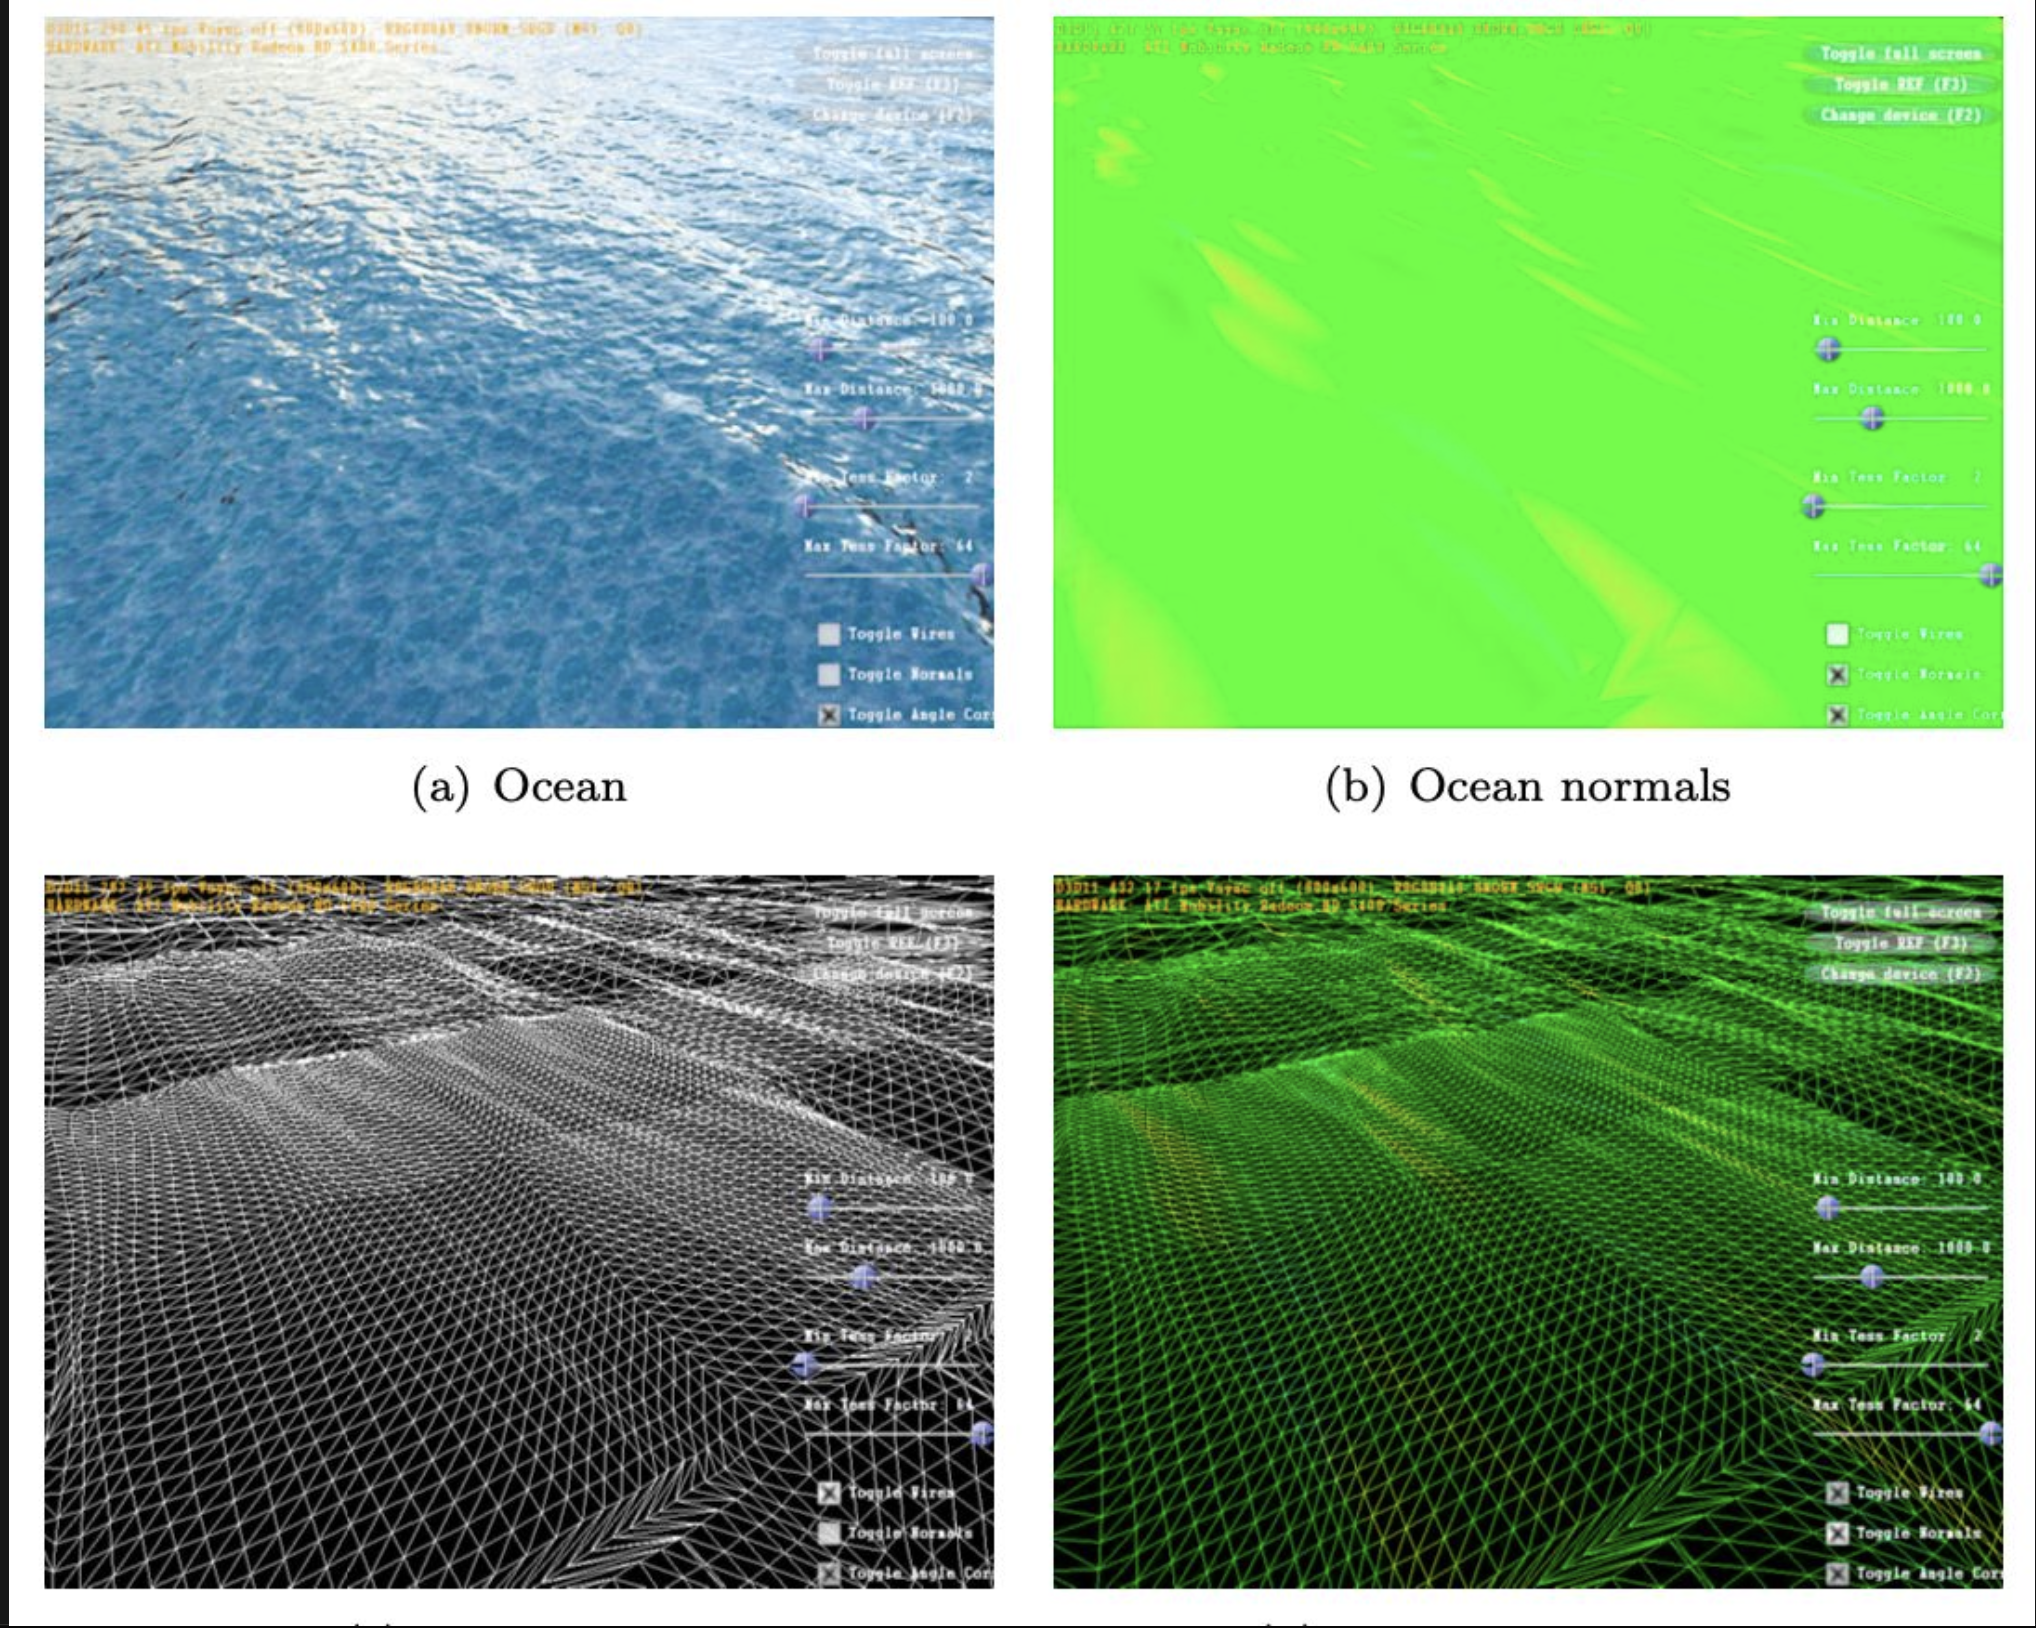
\includegraphics[width=\textwidth]{imgs/terrain-and-water.png}
        
        \column{0.45\textwidth}
        \centering
        \includegraphics[width=\textwidth]{imgs/terrain-and-water-2.png}
    \end{columns}
\end{frame}


%=================================================
\section{Simulação do Empinamento}
%=================================================
\begin{frame}{Simulação do Empinamento}
    \begin{itemize}
        \item O empinamento das ondas é um fenômeno importante na dinâmica oceânica.
        \item A simulação deste processo ajuda a entender como as ondas interagem com estruturas costeiras e como a energia das ondas é dissipada.
    \end{itemize}
\end{frame}

\begin{frame}{Real-time Breaking Waves for Shallow Water Simulations}
        \begin{itemize}
        \item \textbf{Objetivo:} Aprimorar simulações de águas rasas com o efeito de ondas que quebram, utilizando um modelo de campo de altura eficiente para aplicações em tempo real.
        \item \textbf{Desafio:} Simulações 3D de fluidos são computacionalmente caras para aplicações interativas.
        \item \textbf{Solução:} Combinação de simulação de campo de altura (2D) com partículas para representar ondas que quebram.
    \end{itemize}
\end{frame}

\begin{frame}{Simulação de Águas Rasas (Shallow Water - SW)}
    \begin{itemize}
        \item Redução de um problema 3D para uma representação 2D de campo de altura.
        \item A velocidade do fluido não varia significativamente ao longo do eixo z.
        \item As únicas forças que impulsionam o fluido são pressão e gravidade.
        \item Usa as equações de Euler, negligenciando a viscosidade.
        \item As equações simplificadas de águas rasas são:
        \begin{align*}
            H_t &= -u \cdot \nabla H - H(u_x + v_y) \\
            u_t &= -u \cdot \nabla u - gh_x \\
            v_t &= -u \cdot \nabla v - gh_y
        \end{align*}
        \item Onde $H$ é a altura total da água e do terreno, $u$ é a velocidade horizontal do fluido, e $g$ é a força da gravidade.
        \item Vantagens: Fornece um campo de velocidade completo para a superfície e pode ser facilmente estendida com várias condições de contorno.
    \end{itemize}
\end{frame}

\begin{frame}{Geração de Ondas Quebrando}
    \begin{itemize}
        \item \textbf{Detecção:} Identificação de regiões com frentes de ondas íngremes onde a inclinação da altura do fluido é maior que um limiar e a velocidade do fluido se opõe ao gradiente da altura.
        \item \textbf{Critério de Detecção:} $|\nabla H(x)| > t_H$ e $\nabla H(x) \cdot u(x) < 0$, onde $t_H = p_H g \Delta t / \Delta x$.
        \item \textbf{Construção de Linhas de Onda:} Criação de linhas de pontos conectados ao longo da frente da onda.
        \item As linhas são advectadas usando a velocidade da onda e projetadas ao longo do gradiente de altura.
        \item \textbf{Geração de Patches de Fluidos:} Criação de patches de partículas conectadas ao longo da linha da onda para representar a onda quebrando.
        \item A velocidade das partículas do patch é calculada com base na velocidade da linha da onda e na energia potencial.
    \end{itemize}
\end{frame}

\begin{frame}{Demonstração}
    \begin{columns}
        \column{0.45\textwidth}
        \centering
        \includegraphics[width=\textwidth]{imgs/real-time-1.png}
        
        \column{0.45\textwidth}
        \centering
        \includegraphics[width=\textwidth]{imgs/real-time-2.png}
    \end{columns}
\end{frame}

\begin{frame}{Resultados e Desempenho}
    \begin{itemize}
        \item Simulações em tempo real de ondas quebrando com taxas de quadros de 40 a 75 fps em hardware comum.
        \item O modelo permite a criação de ondas em diversas configurações e condições.
        \item A simulação de fluidos representa cerca de 80% do tempo de execução, enquanto a renderização e o overhead do motor gráfico consomem os 20% restantes.
        \item Aproximadamente metade do tempo de simulação é gasto na simulação de águas rasas, e um quarto é gasto no algoritmo de simulação de ondas.
    \end{itemize}
\end{frame}

%=================================================
\section{Referências}
%=================================================
\begin{frame}[allowframebreaks]{Referências}
    \nocite{*}
    \bibliographystyle{plain}
    \bibliography{Bibliografia}
\end{frame}

\end{document}
